\chapter{Experimentos}\label{cap.experimentos}


\par El modelo propuesto de clasificación de ironía se implementó en Python. Este capítulo consiste en presentar, comparar y dar una explicación sobre por que se obtienen dichos resultados, para cada uno de los experimentos se probó con diferentes configuraciones para compararlos entre ellos, con el objetivo de encontrar la que presente mejores resultados.

\section{Primer experimento}

\par En este primer experimento se probó con una arquitectura con una primera capa de embedding de 128 unidades de salida, seguida de una capa \gls{bi-lstm} de 200 unidades, después una capa de dropout con parámetro de 0.5, seguida de una capa completamente conectada con una única salida que representa el resultado binario que indica si la oración es irónica o no. Este experimento se distingue de los demás ya que no tomamos en cuenta los caracteres especiales, únicamente el texto el cual se normaliza a ASCII con el propósito de no darle tanta importancia a la ortografía. Se agrega al final un carácter que delimita si es el final de la sentencia.

\subsection{Evaluación}
\begin{center}
	\begin{table}[h]
    \centering
    \caption{Tabla de métricas experimento 1, análisis por palabra. Nótese que la métrica con valor más alto es la exactitud, con un promedio de 0.9687; sin embargo, el recall cae debido a que no le es posible encontrar más muestras positivas, esto puede deberse a que ignora mucha información valiosa que contienen las palabras que se omiten. La desviación estándar resulta ser muy baja, lo cuál indica que este experimento no varía tanto y por lo tanto los promedios describen el comportamiento esencial del modelo.}
\begin{tabular}{|l|llll|}
\hline
              & Exactitud &     Precisión &     Recall  &   F-score \\ \hline

Subdivisión1            &       0.9698  &       0.9277  &       0.7589  &       0.8349  \\ 
Subdivisión2            &       0.9671  &       0.8422  &       0.8246  &       0.8333  \\ 
Subdivisión3            &       0.9692  &       0.9045  &       0.7720  &       0.8330  \\ 
Subdivisión4            &       0.9677  &       0.9569  &       0.7097  &       0.8150  \\ 
Subdivisión5            &       0.9698  &       0.9146  &       0.7694  &       0.8358  \\ \hline
Promedio                &       0.9687  &       0.9092  &       0.7669  &       0.8304  \\ \hline
Desviación estándar     &       0.0011  &       0.0378  &       0.0366  &       0.0078  \\ \hline

% Subdivisión 1 & 0.9709  &       0.9674  &       0.7226  &       0.8273 \\
% Subdivisión 2 & 0.9677  &       0.9529  &       0.7037  &       0.8095   \\
% Subdivisión 3 & 0.9647  &       0.9711  &       0.6793  &       0.7994   \\
% Subdivisión 4 & 0.9698  &       0.9719  &       0.7333  &       0.8359   \\
% Subdivisión 5 & 0.9722  &       0.9312  &       0.7713  &       0.8437  \\ \hline
% Promedio      & 0.9690  &       0.9589  &       0.7220  &       0.8232\\ \hline
\end{tabular}
		     \label{tab:exp1}
\end{table}
\end{center}

\par Como se puede apreciar en la tabla \ref{tab:exp1} la precisión medida sobre el modelo, es similar a la obtenida en la bibliografía, lo cual indica que este modelo se desempeña bastante bien en reconocer la ironía. Sin embargo, como se vió, el \textit{recall} es considerablemente bajo, por lo que este modelo tiende a no encontrar un gran porcentaje de las muestras irónicas. Ademá se puede ver que el \textit{F-score} es bastante similar a los de la bibliografía.

\vspace{6pt}

\par Como se vio en el capítulo \ref{cap.metodologia}, las gráficas ROC constituyen una buena forma gráfica de evaluar un modelo. A continuación en la figura \ref{fig:Roc1} se muestran algunas de las gráficas ROC qué muestran qué tan bien se desempeña esta arquitectura y preprocesamiento.

\begin{figure}
	\begin{table}[H]
		\centering
		\makebox[10pt][c]{
			\begin{tabular}{cc}

				\addheight{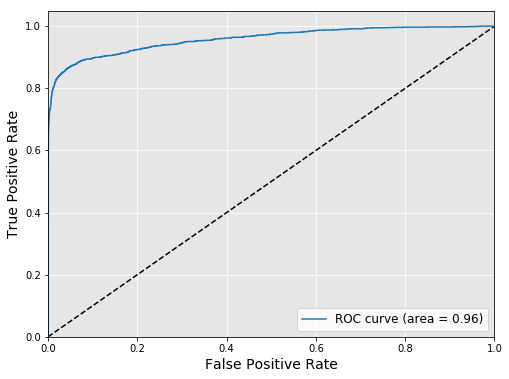
\includegraphics[width=80mm]{imagenes/ROC_Exp1_1.png}} &
				\addheight{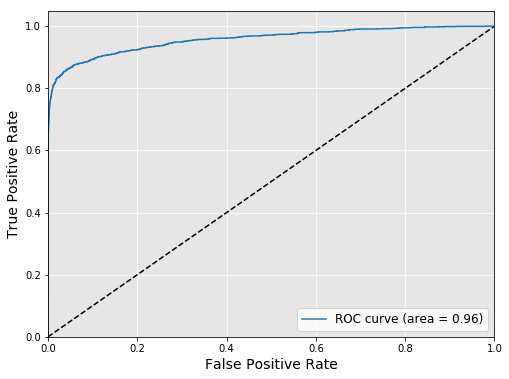
\includegraphics[width=80mm]{imagenes/ROC_Exp1_2.png}}              \\
				\small Segmento 1                                                 & Segmento 2 \\

				\addheight{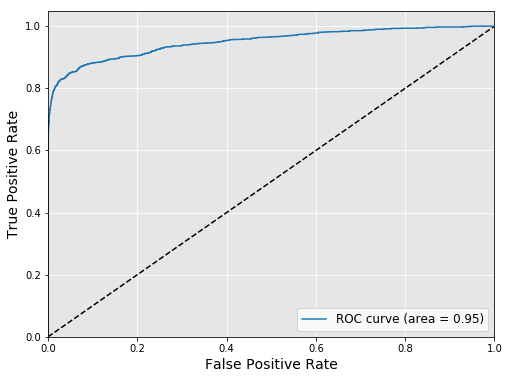
\includegraphics[width=80mm]{imagenes/ROC_Exp1_3.png}} &
				\addheight{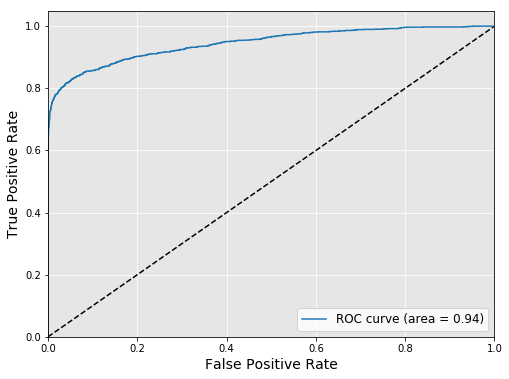
\includegraphics[width=80mm]{imagenes/ROC_Exp1_4.png}}              \\
				\small Segmento 3                                                 & Segmento 4 \\

				\addheight{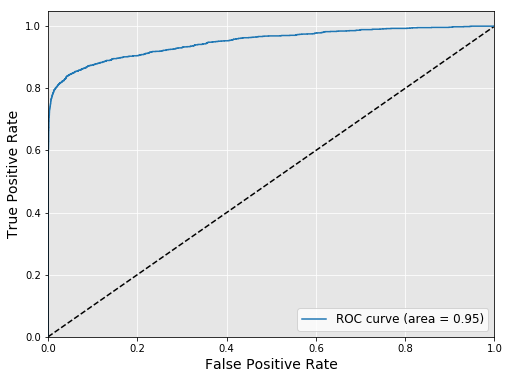
\includegraphics[width=80mm]{imagenes/ROC_Exp1_5.png}} &
				\\
				\small Segmento 5                                                 &            \\
			\end{tabular}
		}
	\end{table}
	\caption{Gráficas ROC de los segmentos en que se dividió el corpus. Primer Experimento preprocesamiento por palabra. En este experimento se puede apreciar como las gráficas ROC tiene un línea más accidentada, lo cual determina que tan estable es el modelo, si se mueve el umbral. El área bajo la curva alcanza 0.96, es un buen resultado, sin embargo, al compararlo con los demás experimentos se puede notar que no es tan relevante.}
	\label{fig:Roc1}
\end{figure}


\subsection{Propuesta de mejora}

\par Mi propuesta de mejora es que en lugar de considerar las palabras como tokens, se consideren los caracteres. Esto podría mejorar el desempeño ya que dejaríamos que la red neuronal aprendiera de la forma que escriben los usuarios y no se esforzaría tanto por encontrar correlaciones con palabras que no se encuentran en una oración. Similar a como los humanos leemos las palabras, ya que podemos extraer características diferentes de dos textos que tienen un contenido similar por ejemplo: `hola' y `holaaaaaaa' en la primera podemos notar que es ortograficamente correcta. No obstante no da mucha información por sí misma, con la segunda podemos ver que no es ortograficamente correcta, por lo que muy probablemente no este en el vocabulario que se extrajo del conjunto de entrenamiento. Si la palabra tiene los últimos caracteres repetidos puede indicar que se quiere hacer algún tipo de énfasis, o que el emisor quiere señalar algo evidente. Estos son ejemplos de características que se pueden obtener si se hace un análisis carácter por carácter y la principal motivación para el siguiente experimento.

\section{Segundo experimento}
\par En este segundo experimento se quiso cambiar el preprocesamiento, realizando lo más sencillo, pasar el tweet a una lista de caracteres y considerar cada uno como unidad de información. Entonces el vocabulario sería cada uno de los caracteres que se encuentran presentes en el corpus distinguiendo si eran mayúsculas o minúsculas. Tampoco se excluyeron los caracteres especiales, para de este modo captar la mayor información posible.
\subsection{Evaluación}
\begin{center}
	\begin{table}[h]
    \centering
    \caption{Tabla de métricas experimento 2, análisis por carácter. Se nota un mejor desempeño respecto al primer experimento, debido a que las palabras que fueron ignoradas antes, ahora aportan su información. La mejor métrica de este experimento fue la exactitud, pero se nota una mejora significativa en la precisión y en el recall, de 5 y 10 puntos porcentuales respectivamente. La desviación estándar resulta ser muy baja, lo cuál indica que este experimento no varía tanto y por lo tanto los promedios describen el comportamiento esencial del modelo. }
\begin{tabular}{|l|llll|}
\hline
                        & Exactitud &     Precisión &     Recall  &   F-score \\ \hline
              
Subdivisión1            &       0.9840  &       0.9450  &       0.8928  &       0.9181  \\ 
Subdivisión2            &       0.9842  &       0.9646  &       0.8737  &       0.9169  \\ 
Subdivisión3            &       0.9811  &       0.9477  &       0.8568  &       0.8999  \\ 
Subdivisión4            &       0.9801  &       0.9562  &       0.8402  &       0.8944  \\ 
Subdivisión5            &       0.9833  &       0.9623  &       0.8674  &       0.9124  \\ \hline
Promedio                &       0.9825  &       0.9552  &       0.8662  &       0.9084  \\ \hline
Desviación estándar     &       0.0016  &       0.0078  &       0.0175  &       0.0095  \\ \hline
              
% Subdivisión 1 & 0.9716  &       0.8911  &       0.8130  &       0.8503 \\
% Subdivisión 2 & 0.9639  &       0.8648  &       0.7557  &       0.8066   \\
% Subdivisión 3 & 0.9768  &       0.8905  &       0.8808  &       0.8857   \\
% Subdivisión 4 & 0.9660  &       0.8683  &       0.7723  &       0.8175   \\
% Subdivisión 5 & 0.9707  &       0.8894  &       0.8096  &       0.8476   \\ \hline
% Promedio      & 0.9698  &       0.8808  &       0.8063  &       0.8415\\ \hline
\end{tabular}
		     \label{tab:exp2}
\end{table}
\end{center}


\par En la tabla \ref{tab:exp2} se puede notar un mejora considerable ya que pasa de tener un 83.04 \% de \textit{F-score} promedio a un 90.84\% . Esto es debido a que se pudieron obtener mejores características de las secuencias de caracteres. A continuación en la figura \ref{fig:Roc2} se muestran algunas de las gráficas ROC que muestran qué tan bien se desempeña este modelo.

\begin{figure}

	\begin{table}[H]
		\centering
		\makebox[10pt][c]{
			\begin{tabular}{cc}

				\addheight{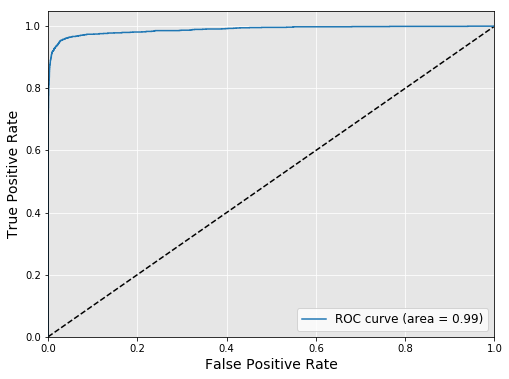
\includegraphics[width=80mm]{imagenes/ROC_Exp2_1.png}} &
				\addheight{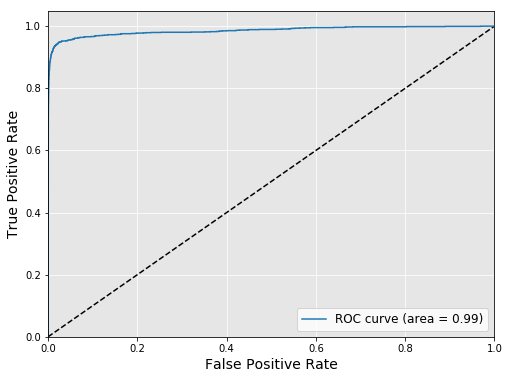
\includegraphics[width=80mm]{imagenes/ROC_Exp2_2.png}}              \\
				\small Segmento 1                                                 & Segmento 2 \\

				\addheight{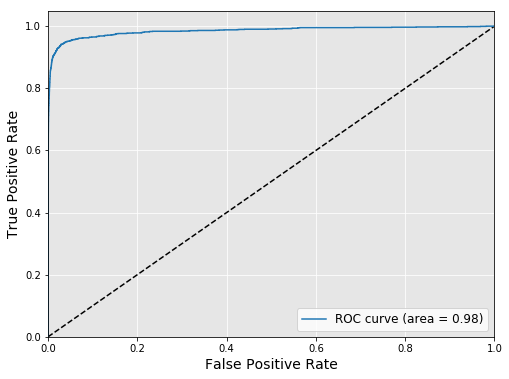
\includegraphics[width=80mm]{imagenes/ROC_Exp2_3.png}} &
				\addheight{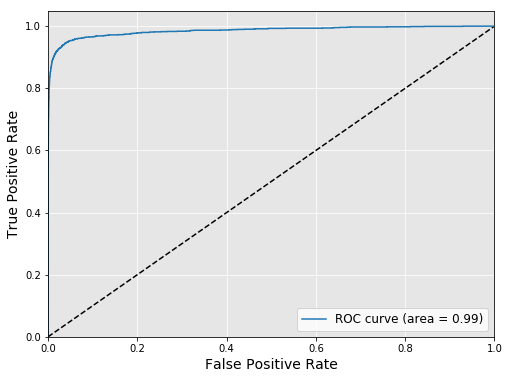
\includegraphics[width=80mm]{imagenes/ROC_Exp2_4.png}}              \\
				\small Segmento 3                                                 & Segmento 4 \\

				\addheight{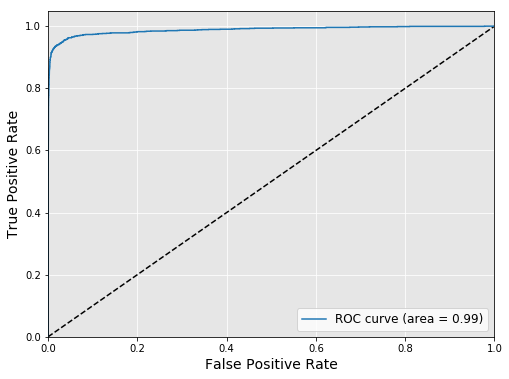
\includegraphics[width=80mm]{imagenes/ROC_Exp2_5.png}} &
				\\
				\small Segmento 5                                                 &            \\
			\end{tabular}
		}

	\end{table}
	\caption{Gráficas ROC de los segmentos en que se dividió el corpus. Segundo experimento por caracteres n-gram  es 1. Se puede notar un crecimiento abrupto al inicio de la gráfica, lo cuál indica que las predicciones se separan más, con respecto al experimento 1. Se puede notar una mejora en el desarrollo de la recta, siendo más suave en la mayoría de las gráficas. Además, hay una mejora significativa en el área bajo la curva, llegando a 0.99.}

	\label{fig:Roc2}
\end{figure}
\par Se puede notar que los segmentos de este experimento están siempre tiene un AUC por encima del máximo del experimento 1. Lo cual indica directamente que es un mejor modelo.

\subsection{Propuesta de mejora} 

\par Al analizar los resultados obtenidos se pudo observar una mejora considerable, tanto el \textit{recall} como en \textit{precision} lo que indica que este modelo es mucho mejor que el primero. Esto puede ser debido a que en las redes sociales las reglas gramaticales y de ortografía son más flexibles, y para poner un ejemplo: escribir
``hola ¿Que haces?'' es lo mismo que decir ``ola k ase'', semanticamente hablando, por lo que analizando palabra por palabra la similitud entre estas palabras es pequeña mientras que carácter por carácter es más grande debido a la red neuronal puede encontrar secuencias de caracteres que realmente importa como `ola'  y también encontrar una correlación entre `que' y `k' lo cual significaría que se adapta al uso de la lengua.

\par El \textit{recall} como se explicó previamente es la medida que indica qué porcentaje de muestras relevantes es encontrada. Los números indican que en el experimento 1 de 100 muestras irónicas, pudo distinguir 76 y en el experimento 2 pudo distinguir 86. Mientras que el \textit{precision} es la medida que muestra que porcentaje de las muestras clasificadas como irónicas fue de verdad irónica. Por lo tanto en números el experimento 1 detectó 100 muestras irónicas, de las cuales el 90.92 \% fue de verdad irónica y el experimento 2 de 100 detectó 95.52 \% irónicas. En ambas métricas el segundo experimento es mucho mejor.

\par Con el fin de mejorar este resultado se propone aumentar el tamaño del n-gram a dos. Esto aportaría mayor información de la vecindad de los caracteres, pudiendo encontrar mejores patrones que describan más globalmente la esencia de los datos.

\section{Tercer Experimento}
\par En este experimento se incrementó el tamaño de los tokens ahora serán tomados por parejas de caracteres. Por lo que algunos tokens podrían ser los siguientes: `ho', `ol', `la'. Lo que se busca con este experimento es obtener más flexibilidad que cuando procesa por palabra y mayor rigidez que cuando procesa por carácter. Los resultados fueron los siguientes:

\subsection{Evaluación}
\begin{center}
	\begin{table}[h]
    \centering
    \caption{Tabla de métricas experimento 3, análisis por tupla de dos caracteres. Se puede notar una mejora en el valor del reclamo, 0.8958 promedio, lo cual eleva el valor-F a 0.9157 promedio, la desviación estándar se mantiene, aumentando un poco en la precisión y disminuyendo en el reclamo, pero aún así es baja por lo que puede considerarse estable. }
\begin{tabular}{|l|llll|}
\hline
& Exactitud &     Precisión &     Reclamo  &   Valor-F \\ \hline
              
Subdivisión1            &       0.9828  &       0.9311  &       0.8954  &       0.9129  \\ 
Subdivisión2            &       0.9842  &       0.9362  &       0.9031  &       0.9194  \\ 
Subdivisión3            &       0.9824  &       0.9076  &       0.9159  &       0.9117  \\ 
Subdivisión4            &       0.9831  &       0.9436  &       0.8845  &       0.9131  \\ 
Subdivisión5            &       0.9850  &       0.9670  &       0.8798  &       0.9213  \\ \hline
Promedio                &       0.9835  &       0.9371  &       0.8958  &       0.9157  \\ \hline
Desviación estándar     &       0.0010  &       0.0192  &       0.0130  &       0.0039  \\ \hline

% Subdivisión 1 & 0.9793 &   0.9387 &   0.8466 &   0.8903  \\
% Subdivisión 2 & 0.9712 &   0.8597 &   0.8490 &   0.8543  \\
% Subdivisión 3 & 0.9743 &   0.9478 &   0.7912 &   0.8624  \\
% Subdivisión 4 & 0.9686 &   0.9221 &   0.7445 &   0.8239  \\
% Subdivisión 5 & 0.9775 &   0.9199 &   0.8506 &   0.8839  \\ \hline
% Promedio      & 0.9742 &  0.9176 &  0.8164 &  0.8630\\ \hline
\end{tabular}
		     \label{tab:exp3}
\end{table}
\end{center}

\par En la tabla \ref{tab:exp3} se puede ver una mejora leve con respecto al experimento anterior con un promedio de \textit{F-score} de 91.57 \% un aumento de casi 1 \%. A continuación en la figura \ref{fig:Roc3}  se muestran algunas de las gráficas ROC que muestran qué tan bien se desempeña este algoritmo.

\begin{figure}

	\begin{table}[H]
		\centering
		\makebox[10pt][c]{
			\begin{tabular}{cc}

				\addheight{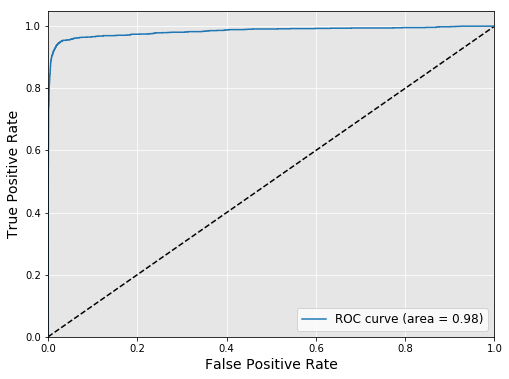
\includegraphics[width=80mm]{imagenes/ROC_Exp3_1.png}} &
				\addheight{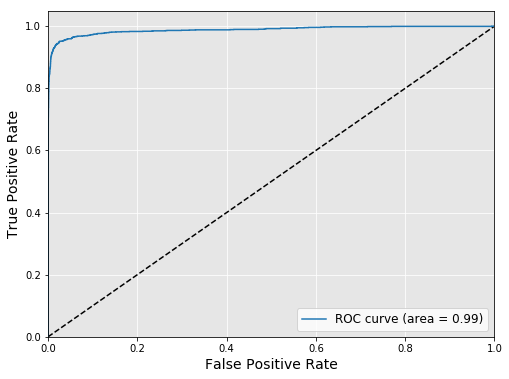
\includegraphics[width=80mm]{imagenes/ROC_Exp3_2.png}}              \\
				\small Segmento 1                                                 & Segmento 2 \\

				\addheight{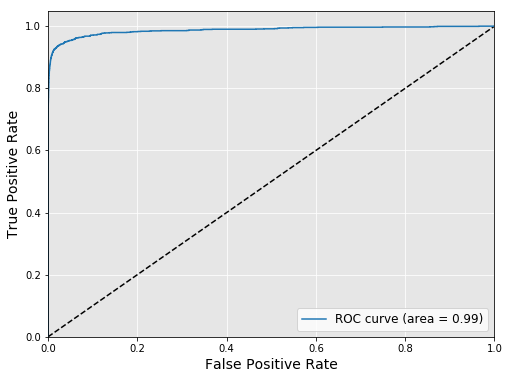
\includegraphics[width=80mm]{imagenes/ROC_Exp3_3.png}} &
				\addheight{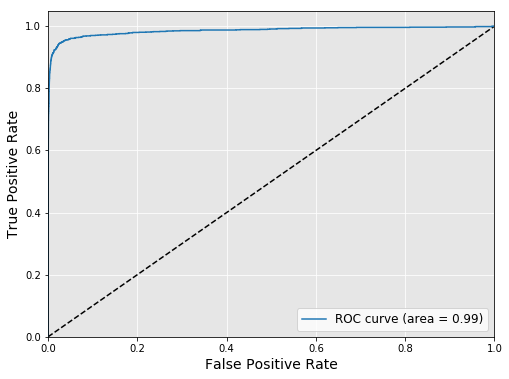
\includegraphics[width=80mm]{imagenes/ROC_Exp3_4.png}}              \\
				\small Segmento 3                                                 & Segmento 4 \\

				\addheight{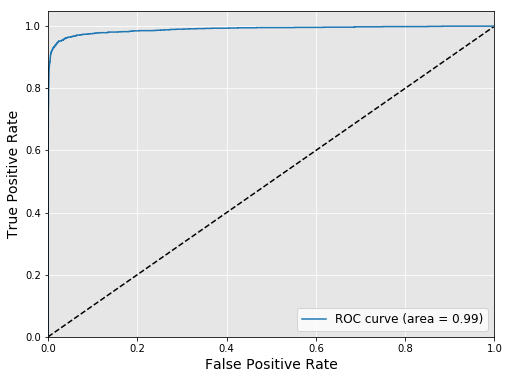
\includegraphics[width=80mm]{imagenes/ROC_Exp3_5.png}} &
				\\
				\small Segmento 5                                                 &            \\
			\end{tabular}
		}

	\end{table}
	\caption{Gráficas ROC de los segmentos en que se dividió el corpus. Tercer experimento por caracteres n-gram  es 2. Se puede notar una mejora sutíl con respecto al segundo experimento. Cabe destacar que el segmento 1 tiene una desarrollo más accidentado, el cuál puede notarse igualmente en experimento dos; esto puede deberse a que la distribución de las muestras es más desfavorable para ese segmento. El área bajo la curva se mantiene en 0.99 y sólo la del segmento 1 es 0.98.}
	\label{fig:Roc3}
\end{figure}



\subsection{Análisis}
\par En este experimento se pudo notar una mejora leve con respecto a los resultados previos. Se pudo ver que los resultados de \textit{accuracy}, \textit{recall} y \textit{f-score} mejoran con respecto al segundo experimento, lo que indica directamente que es un mejor modelo. Sin embargo, la única métrica que no mejora es la \textit{precision} lo que indica que de las muestras que reconoce como irónicas el segundo experimento tiene menores probabilidades de equivocarse. Sin embargo, también tiene menores probabilidades de encontrar las muestras irónicas (\textit{recall}). Y si consideramos el promedio de las dos métricas, se comporta mejor este modelo que el primero.

\par Como propuesta para siguientes experimentos, puede aumentarse el tamaño del n-gram para tratar de encontrar un punto medio que mejore estas métricas, aunque probablemente ya se haya encontrado o esté por encontrarse.

\begin{figure}
	\centering
	
\includegraphics[width=0.7\textwidth]{imagenes/ironia1.png}
	\caption{Texto irónico tomado a prueba. En esta muestra se obtuvo un 0.997028 de porcentaje de ironía. Para el experimento 3.} %%%ACTUALIZAR
	\label{fig:ironyTest1}
\end{figure}

\begin{figure}
	\centering
	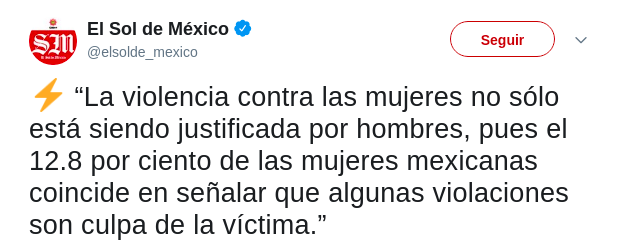
\includegraphics[width=0.7\textwidth]{imagenes/ironia2.png}
	\caption{Texto no irónico tomado a prueba. En esta muestra se obtuvo un 0.0135374 de porcentaje de ironía. Para el experimento 3} %%%ACTUALIZAR
	\label{fig:ironyTest2}
\end{figure}

\par En la figura \ref{fig:ironyTest1} se puede ver que es una muestra irónica que tiene un alto porcentaje de predicción y en la segunda figura \ref{fig:ironyTest2} se puede ver que no es un texto irónico y presenta un bajo porcentaje de predicción. En estas ejemplos se puede ver como se la predicción que hace el sistema.

\section{Cuarto Experimento}

\par En este experimento se probo aumentar el tamaño de la palabra de n-gram, esto con el fin de obtener una mayor flexibilidad que usando como tokens las palabras y una mayor rigidez que cuando se usa n-gram de dos.

\subsection{Evaluación}

\begin{center}
	\begin{table}[h]
	\centering
	\caption{Tabla de métricas experimento 4, por tuplas de 3 caracteres. En esta tabla se puede ver una disminución considerable del F-score, pero un aumente en el recall, además de una disminución en la desviación estándar, lo cual indica que es más estable, en cuando a recall. La precisión cae abruptamente y aumenta considerablemente su desviación estándar.}
\begin{tabular}{|l|llll|}
\hline
& Exactitud &     Precisión &     Recall  &   F-score \\ \hline
              
Subdivisión1            &       0.9754  &       0.8687  &       0.8895  &       0.8790  \\ 
Subdivisión2            &       0.9294  &       0.5959  &       0.9110  &       0.7205  \\ 
Subdivisión3            &       0.8768  &       0.4436  &       0.9409  &       0.6029  \\ 
Subdivisión4            &       0.9364  &       0.6259  &       0.9080  &       0.7410  \\ 
Subdivisión5            &       0.9507  &       0.7014  &       0.8837  &       0.7821  \\ \hline
Promedio                &       0.9338  &       0.6471  &       0.9066  &       0.7451  \\ \hline
Desviación estándar     &       0.0325  &       0.1389  &       0.0200  &       0.0896  \\ \hline



% Subdivisión 1 & 0.9800 & 0.9450 & 0.8479 & 0.8938  \\
% Subdivisión 2 & 0.9787 & 0.9340 & 0.8457 & 0.8877  \\
% Subdivisión 3 & 0.9788 & 0.9414 & 0.8443 & 0.8902  \\
% Subdivisión 4 & 0.9720 & 0.8247 & 0.9093 & 0.8650  \\
% Subdivisión 5 & 0.9743 & 0.8452 & 0.9116 & 0.8771  \\ \hline
% Promedio      & 0.9768 & 0.8718 & 0.8981 & 0.8828  \\ \hline
\end{tabular}
		     \label{tab:exp4}
\end{table}
\end{center}

\par Se puede notar en la tabla \ref{tab:exp4} que el \textit{f-score} es el peor de todos los experimentos, lo cual indica que el equilibrio que se buscaba al aumentar el n-gram ya se había alcanzado con el tercer experimento.

\par Sin embargo, un punto a recalcar en este experimento es que su medida de \textit{recall} es la mejor de los 4 experimentos. Lo cual sería importante si fuera uno de esos problemas en lo que es más importante predecir la mayor parte de las muestras positivas aunque haya muchas veces falsas alarmas, como en sismos, desastres naturales, etc.

\par A continuación en la figura \ref{fig:Roc4}  se muestran algunas de las gráficas ROC que muestran qué tan bien se desempeña este algoritmo. En estas gráficas se puede ver que son peores que la de cualquier experimento, pero siguen teniendo una buena área bajo la curva, lo que indica que es un experimento bastante bueno.

\begin{figure}

	\begin{table}[H]
		\centering
		\makebox[10pt][c]{
			\begin{tabular}{cc}

				\addheight{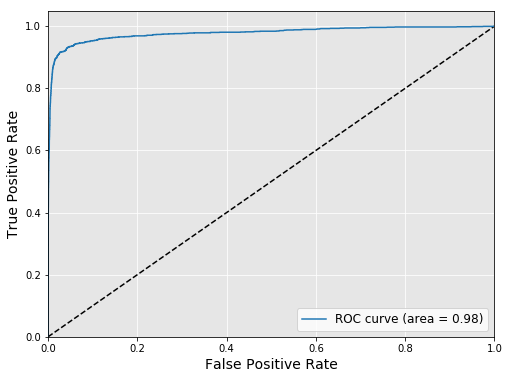
\includegraphics[width=80mm]{imagenes/ROC_Exp4_1.png}} &
				\addheight{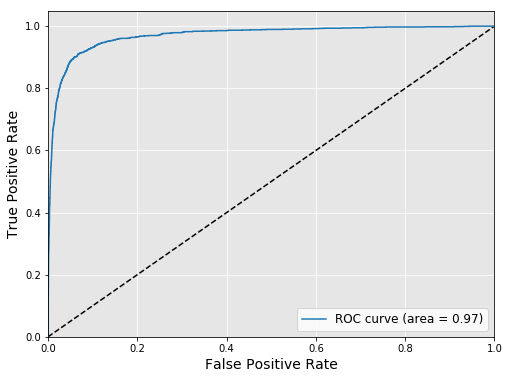
\includegraphics[width=80mm]{imagenes/ROC_Exp4_2.png}}              \\
				\small Segmento 1                                                 & Segmento 2 \\

				\addheight{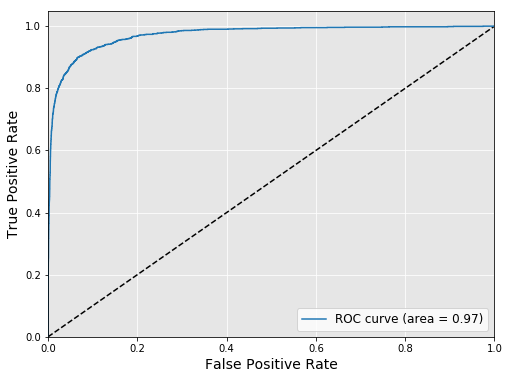
\includegraphics[width=80mm]{imagenes/ROC_Exp4_3.png}} &
				\addheight{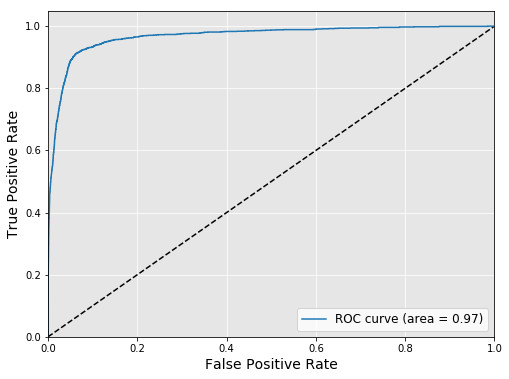
\includegraphics[width=80mm]{imagenes/ROC_Exp4_4.png}}              \\
				\small Segmento 3                                                 & Segmento 4 \\

				\addheight{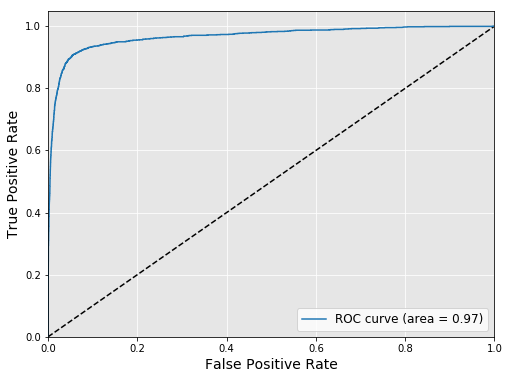
\includegraphics[width=80mm]{imagenes/ROC_Exp4_5.png}} &
				\\
				\small Segmento 5                                                 &            \\
			\end{tabular}
		}

	\end{table}
	\caption{Gráficas ROC de los segmentos en que se dividió el corpus. Cuarto experimento por caracteres n-gram  es 3. Se puede notar una desmejora, general con respecto a los dos experimentos anteriores. Comparado con el experimento 1, este tiene un desarrollo de la recta más suave, lo qué indica que tiene un comportamiento más estable, si se mueve el umbral. El área bajo la curva alcanza a lo más 0.98.}
	\label{fig:Roc4}
\end{figure}

\par En la figura \ref{fig:ironyTest3} y \ref{fig:ironyTest4} se pueden ver ejemplos de cómo el modelo del experimento 4 detecta una muestra irónica y otra que no es irónica.

\begin{figure}[h]
	\centering
	
\includegraphics[width=0.6\textwidth]{imagenes/ironia3.png}
	\caption{Texto medianamente irónico tomado a prueba. En esta muestra se obtuvo un 0.87694 de porcentaje de ironía. Para el experimento 4.} %%%ACTUALIZAR
	\label{fig:ironyTest3}
\end{figure}

\begin{figure}[h]
	\centering
	
\includegraphics[width=0.6\textwidth]{imagenes/ironia4.png}
	\caption{Texto no irónico tomado a prueba. En esta muestra se obtuvo un 0.00296568 de porcentaje de ironía. Para el experimento 4} %%%ACTUALIZAR
	\label{fig:ironyTest4}
\end{figure}







\section{Análisis}
\par Para concluir este capítulo se muestra una tabla que compara directamente las diferentes medidas obtenidas en esta fase de experimentos.

\begin{center}
	\begin{table}[H]
		\centering
		
\begin{tabular}{|l|llll|}
\hline
\# Experimento & Accuracy &     Precision &     Recall  &   F1-score \\ \hline
Experimento 1 (palabras) &       0.9687  &       0.9092  &       0.7669  &       0.8304  \\ \hline
Experimento 2 (1-gram) &       0.9825  &       {\color{OliveGreen} 0.9552}  &       0.8662  &       0.9084  \\ \hline
Experimento 3 (2-gram) &       {\color{OliveGreen} 0.9835}  &       0.9371  &       0.8958  &       {\color{OliveGreen} 0.9157}  \\ \hline
Experimento 4 (3-gram) &       0.9338  &       0.6471  &      {\color{OliveGreen}  0.9066}  &       0.7451  \\ \hline
\end{tabular}
\caption{Tabla total de métricas.}

		\label{tab:total}
	\end{table}
\end{center}

\par En esta tabla se puede notar que el tercer experimento de 2-gram tiene dos métricas mejor que cualquier otro experimento, la primera es el \textit{accuracy} con un 98.35\% y el \textit{F-score} de 91.57\% lo cual está indicando se comporta en general como un mejor modelo que cualquiera de los otros 3. Sin embargo, en el \textit{recall} se puede ver que es mejor el del cuarto experimento, llegando a 90.66\% lo cual como se mencionó puede ser mejor en algunos casos que sea muy importante encontrar la mayor parte de las muestras positivas; sin embargo, su \textit{precision} cae abruptamente. Hablando del \textit{precision} se puede ver que es mejor el segundo experimento, sin dejar caer tanto el \textit{recall} por lo que sería un mejor modelo en un caso en el que se requiera obtener una gran parte de muestras positivas sin disparar tantas falsas alarmas.

